\documentclass[compress,xcolor=table]{beamer}
\usepackage[T1]{fontenc}

\usepackage{etoolbox}
\usepackage{ragged2e}
\usepackage{multicol}

%\usepackage{times}
%\renewcommand{\ttdefault}{cmtt}

\usepackage[normalem]{ulem}

\usepackage{tikz}
\usetikzlibrary{shapes}
\usetikzlibrary{arrows}
\usetikzlibrary{patterns}

\usetikzlibrary{external}
\tikzsetexternalprefix{../}

%\tikzexternalize[shell escape=-enable-write18]
%\tikzset{external/system call={lualatex \tikzexternalcheckshellescape -halt-on-error -interaction=batchmode -jobname "\image" "\texsource"}}
%\tikzset{external/force remake}

\usepackage{pgfplots}
\pgfplotsset{compat=newest}
\pgfplotsset{plot coordinates/math parser=false}

\usepackage{pgfplotstable}
\pgfplotstableset{set thousands separator ={}}
\usepackage{booktabs}

\usepackage[simplified,nocolor]{../pgf-umlcd}

\usepackage{booktabs}
\usepackage{multirow}

\usepackage{../IEEEtrantools}

\usepackage{algpseudocode}

%============================================================================
% commands.tex
%============================================================================
% This file contains:
% 	- Defined Variables
%	- Redefined math shorthand
%	- Defined math shorthand

%============================================================================
% Defined Variables
%============================================================================
% 	- \abstractType:
%		Use: Toggles the type of abstract to be used
%		Default Value: abstract
%		Options: abstract, umiabstract
\newcommand{\abstractType}{abstract}

%============================================================================
% Redefined Math Commands
%============================================================================
% 	- \Vec{1} or \vec{1}
%		Long Name: Vector
%		Arguements[1]: bold and overbar arg1	
\DeclareRobustCommand{\Vec}[1]{%
    \ifmmode
        \mathbf{#1}\,%
    \else
        $\displaystyle \mathbf{#1}\,$%
    \fi
}
\DeclareRobustCommand{\vec}[1]{\Vec{#1}}

\DeclareRobustCommand{\lbm}{%
    \ifmmode
        \text{lb}_{\text{m}}
    \else
        $\displaystyle \text{lb}_{\text{m}}$%
    \fi
}
\DeclareRobustCommand{\lbf}{%
    \ifmmode
        \text{lb}_{\text{f}}
    \else
        $\displaystyle \text{lb}_{\text{f}}$
    \fi
}
\DeclareRobustCommand{\dt}{%
	\ifmmode
		\Delta t
	\else
		$Delta t$
	\fi
}
\DeclareRobustCommand{\dtmax}{%
	\ifmmode
		\Delta t_{\text{MAX}}
	\else
		$\Delta t_{\text{MAX}}$
	\fi
}
\DeclareRobustCommand{\dx}{%
	\ifmmode
		\Delta x
	\else
		$\Delta x$
	\fi
}

\delimitershortfall-1sp
\newcommand\abs[1]{\left|#1\right|}

\DeclareRobustCommand{\BlackBox}{\State \textbf{Black Box: }}
\DeclareRobustCommand{\Test}{\State \textbf{Test: }}
\DeclareRobustCommand{\Define}{\State \textbf{Define: }}
\DeclareRobustCommand{\Update}{\State \textbf{Update: }}
\DeclareRobustCommand{\Set}{\State \textbf{Set: }}
\DeclareRobustCommand{\Calculate}{\State \textbf{Calculate: }}
%\newcommand{\algorithmicset}{\textbf{Set:}}
%\algnewcommand\Solve{\item[\algorithmicset]}
\tikzstyle{Decision} = [diamond, draw, text width=4.5em, text badly centered, node distance=3cm, inner sep=0pt]
\tikzstyle{Action} = [rectangle, draw,text width=5em, text centered, node distance=3cm, rounded corners, minimum height=0em]
\tikzstyle{NodePoint} = [circle, draw, minimum height = 0 em, node distance = 3 cm]
\tikzstyle{BlackBox} = [rectangle, draw, text centered, node distance=1cm, fill=black!10]
\tikzstyle{line} = [draw, -latex']
    

\renewcommand{\fileprefix}[1]{../#1}
\newlength{\hpw}
\setlength{\hpw}{0.5\textwidth}

\usetheme{Szeged}
\usecolortheme{beaver}
\usefonttheme{serif}
%\setbeamertemplate{navigation symbols}{}

%----------------------------------------------------------------------------
%----------------------------------------------------------------------------
\title[Department of Nuclear Engineering and Engineering Physics]{Selective Nonlinear Refinement For
Thermal-Hydraulic Safety Analysis Codes}
\author[Lloyd]{Lewis John Lloyd}
\institute[University of Wisconsin - Madison]
{
  Department of Nuclear Engineering and Engineering Physics \\
  University of Wisconsin - Madison
}
\date[Prelim Defense 2012]{Preliminary Report, 2012}
\subject{Nuclear Engineering}

%----------------------------------------------------------------------------
%----------------------------------------------------------------------------

\begin{document}
%------------------------------------------------------------------------------
%------------------------------------------------------------------------------

%\AtBeginSubsection[]
%{
%\begin{frame}
%\tableofcontents[subsectionstyle=show/shaded/hide,sectionstyle=show/shaded]
%\end{frame}
%}

%------------------------------------------------------------------------------
%------------------------------------------------------------------------------
\frame{\titlepage}
%------------------------------------------------
%------------------------------------------------
\begin{frame}
\frametitle{Introduction}

\textbf{Objective}: Simulate the thermal-hydraulic behavior of a reactor core during postulated accidents more accurately with minimal additional computational cost.

\textbf{Motivation}:
\begin{itemize}
\item{Health and safety of the public}
\item{Safety analysis report}
\item{Emergency core cooling during loss-of-coolant accidents}
\end{itemize}

\textbf{Context}:
\begin{itemize}
\item{COBRA subchannel analysis software
\begin{itemize}
\item{Detailed multi-phase fluid dynamics.}
\end{itemize}
}
\end{itemize}

\end{frame}
%------------------------------------------------
%------------------------------------------------
\begin{frame}

\begin{columns}
\column{\hpw}
\begin{itemize}
\item{\textbf{Background}
\begin{itemize}
\item{Two-Phase Flow}
\item{Computational Geometry}
\item{Numeric Approximations}
\item{Solution Methods}
\item{Research Objectives}
\end{itemize}
}
\end{itemize}

\column{\hpw}
\begin{itemize}
\item{\textbf{Preliminary Work}
\begin{itemize}
\item{Nonlinear COBRA-TF}
\item{Operator-based Scaling}
\item{Numerical Experiments}
\end{itemize}
}
\item{\textbf{Proposed Work}
\begin{itemize}
\item{Scaling}
\item{Domain Decomposition}
\item{Testing}
\end{itemize}
}
\end{itemize}

\end{columns}
\end{frame}
%------------------------------------------------------------------------------
%------------------------------------------------------------------------------
\section[Background]{Background}
%------------------------------------------------------------------------------
%------------------------------------------------------------------------------
\subsection[Two-Phase Flow]{Two-Phase Flow}
%------------------------------------------------
%------------------------------------------------
\begin{frame}
\frametitle{Two-Phase Flow}

\begin{itemize}
\item{Three water fields: vapor, continuous liquid, and dispersed liquid.}
\item{\Ncg{} field.}
\item{Assumptions}
\item{For one-dimensional problems there are nine partial differential equations.
\begin{itemize}
\item{Four conservation of mass equations: \Ncg{} field, water vapor field, continuous liquid field, and entrained liquid field.}
\item{Three conservation of momentum equations: Gaseous phase, continuous liquid field, and entrained liquid field.}
\item{Two conservation of energy equations: Gaseous phase and liquid phase.}
\end{itemize}
}
\end{itemize}

\end{frame}
%------------------------------------------------
%------------------------------------------------
\begin{frame}
\frametitle{Two-Phase Flow: Conservation of Continuous Liquid Field Mass and Momentum and Total Liquid Phase Energy}

\begin{IEEEeqnarray}{rcl}
\frac{\partial \left(\alpha_l \rho_l \right)}{\partial t } & = & -\nabla \cdot \left( \alpha_l \rho_l \vec{u}_l \right) -(1-\eta)\dot{\Gamma}^{'''} - \dot{\Upsilon}^{'''} + \dot{s}^{'''}_{m,l} \nonumber \\
\frac{\partial \left( \alpha_l \rho_l \vec{u}_l \right )}{\partial t } & = & -\nabla \cdot \left( \alpha_l \rho_l \vec{u}_l \vec{u}_l \right) -\alpha_l \nabla P + \alpha_l \rho_l \vec{g} - \vec{\tau}^{'}_{w,l} \nonumber \\
 & + & \vec{\tau}^{'}_{i,gl} - (1 - \eta)\dot{\Gamma}^{'''}\vec{u}^{'} - \dot{\Upsilon}^{'''}\vec{u}^{'} + \dot{s}^{'''}_{p,l} \nonumber \\
\frac{\partial \left( (1 - \alpha_g) \rho_l h_l \right) }{\partial t } & = & -\nabla \cdot \left( \alpha_l \rho_l h_l \vec{u}_l \right) - \nabla \cdot \left( \alpha_e \rho_l h_l \vec{u}_e \right) \nonumber \\
 & - & \dot{\Gamma}^{'''} h^{'}_l +  \dot{q}^{'''}_{i,l} - \dot{q}^{'''}_{n,l}  + \dot{q}^{'''}_{w,l} + (1 - \alpha_g) \frac{\partial P}{\partial t} + \dot{s}^{'''}_{e,l} \nonumber
\end{IEEEeqnarray}

\end{frame}
%------------------------------------------------------------------------------
%------------------------------------------------------------------------------
\subsection[Computational Geometry]{Computational Geometry}
%------------------------------------------------
%------------------------------------------------
\begin{frame}
\frametitle{Computational Geometry}
\begin{columns}
\column{0.65\textwidth}

\begin{itemize}
\item{Sections
\begin{itemize}
\item{Contain subchannels}
\item{Defines spatial discretization of subchannel within section.}
\item{Splitting and merging of subchannels occur at section boundaries.}
\end{itemize}
}
\item{Subchannels
\begin{itemize}
\item{Defines cross-sectional areas.}
\end{itemize}
}
\item{Gaps
\begin{itemize}
\item{Connect subchannel within a section.}
\item{Defines transverse length.}
\end{itemize}
}
\end{itemize}

\column{0.35\textwidth}
\begin{figure}[t]
\centering
\resizebox{!}{0.7\textheight}{
\tikzsetnextfilename{images/complex_geometry_pdf}
\begin{tikzpicture}
%\draw [thick] (-2,-2) rectangle (-1,2);
%\draw [thick] (1,-2) rectangle (2,2);
%\draw [thick] (-0.5,3) rectangle (0.5,7);
%\draw [thick] (-0.5,-7) rectangle (0.5,-3);

%Section 1
\draw [thick] (-0.25,-6) rectangle (0.25,-5.25);
\draw [thick] (-0.4,-5.25) rectangle (0.4,-4.5);
\draw [thick] (-0.5,-4.5) rectangle (0.5,-3.75);
\draw [thick] (-0.3,-3.75) rectangle (0.3,-3);

%Section 2: left then right
\draw [thick] (-1.75,-2) rectangle (-1.25,-1);
\draw [thick] (-1.6,-1) rectangle (-1.4,0);
\draw [thick] (-2,-0) rectangle (-1,1);
\draw [thick] (-1.75,1) rectangle (-1.25,2);

\draw [thick] (1.1,-2) rectangle (1.9,-1);
\draw [thick] (1.1,-1) rectangle (1.9,0);
\draw [thick] (1.25,0) rectangle (1.75,1);
\draw [thick] (1.3,1) rectangle (1.7,2);

%Section 3
\draw [thick] (-0.25,3) rectangle (0.25,3.8);
\draw [thick] (-0.5,3.8) rectangle (0.5,4.6);
\draw [thick] (-0.4,4.6) rectangle (0.4,5.4);
\draw [thick] (-0.5,5.4) rectangle (0.5,6.2);
\draw [thick] (-0.25,6.2) rectangle (0.25,7);
\draw [thick] (-0.25,7) rectangle (0.25,7.8);

%Flow lines
\draw [dashed] (-1.5,2.5) -- (1.5,2.5);
\draw [dashed](-1.5,-2.5) -- (1.5,-2.5);
\draw [dashed,<-] (0,3) -- (0,2.5);
\draw [dashed,->] (-1.5,2.5) -- (-1.5,2);
\draw [dashed,->] (1.5,2.5) -- (1.5,2);
\draw [dashed,->] (0,-2.5) -- (0,-3);
\draw [dashed,<-] (-1.5,-2) -- (-1.5,-2.5);
\draw [dashed,<-] (1.5,-2) -- (1.5,-2.5);

\draw [dashed, <->] (-1.25,-1.5) -- (1.1,-1.5);
\draw [dashed, <->] (-1.4,-0.5) -- (1.1,-0.5);
\draw [dashed, <->] (-1,0.5) -- (1.25,0.5);
\draw [dashed, <->] (-1.25,1.5) -- (1.3,1.5);	
\foreach \y/\ytext in {-4.5/ 1,0/ 2,5.5/ 3}
	\draw (2,\y) node [anchor=west] {Section $\ytext$};
\end{tikzpicture}
}
\end{figure}

\end{columns}

\end{frame}
%------------------------------------------------------------------------------
%------------------------------------------------------------------------------
\subsection[Numeric Approximations]{Numerical Approximations}
%------------------------------------------------
%------------------------------------------------
\begin{frame}
\frametitle{Spatial Approximations}

\begin{columns}
\column{\hpw}

\begin{itemize}
\item{Staggered Grid:
\begin{itemize}
\item{Continuity volumes: mass and energy conservation equations}
\item{Momentum flow paths: momentum conservation equations}
\end{itemize}
}
\item{Conserved quantities are constant over their respective volumes.}
\item{1st Order upwind at volume edges.}
\end{itemize}


\column{\hpw}
\begin{figure}
\centering
\resizebox{\textwidth}{!}{
\tikzsetnextfilename{images/staggered_mesh_eps}
\begin{tikzpicture}
\draw (-3,0) rectangle +(1,5);
\draw (0,0) rectangle +(1,1) (0,1) rectangle +(1,1) (0, 2) rectangle +(1,1) (0,3) rectangle +(1,1) (0,4) rectangle +(1,1);
\draw[dashed] (3,-0.5) rectangle +(1,1) (3,0.5) rectangle +(1,1) (3,1.5) rectangle +(1,1) (3, 2.5) rectangle +(1,1) (3,3.5) rectangle +(1,1) (3,3.5) rectangle +(1,1) (3, 4.5) rectangle +(1,1) ;
\draw[dashed] (-3,0) -- (4,0);
\draw[dashed] (-3,5) -- (4,5);
\draw (-2.5,-1) node {Channel};
\draw (0.5,-1) node {Continuity};
\draw (0.5,-1.5) node {Volume};
\draw (3.5,-1) node {Momentum};
\draw (3.5,-1.5) node {Flow Path};
\end{tikzpicture}
}
\end{figure}
\end{columns}

\end{frame}

%------------------------------------------------
%------------------------------------------------
\begin{frame}
\frametitle{Methods for Nuclear Thermal Hydraulic Safety Analysis}

\begin{itemize}
\item{Fully Explicit Method [COBRA-I]}
\item{Fully Implicit Method [CATHARE] (Barre and Bernard, 1990)}
\item{Semi-Implicit Method [COBRA-TF] (Liles and Reed, 1978) }
\item{Stability-Enhancing Two-Step Method (SETS) [TRACE] (Mahaffy, 1982) }
\item{Nearly Implicit Method [RELAP] (Trapp and Riemke, 1986) }
\end{itemize}

\end{frame}
%------------------------------------------------
%------------------------------------------------
\begin{frame}
\frametitle{Single Newton Step vs. Iterative Newton Method}

\begin{itemize}
\item{Single Newton Step
\begin{itemize}
\item{Linearized Approximation.}
\item{Timestep acceptance based upon error mitigation and prevention.}
\item{Limits placed upon changes in independent parameters.}
\end{itemize}
}
\item{Iterative Newton Step
\begin{itemize}
\item{Nonlinearly Convergent.}
\end{itemize}
}
\end{itemize}

\begin{figure}[t]
\centering
\resizebox{1.0\textwidth}{!}{
\tikzsetnextfilename{images/mySimpleDiagram_pdf}
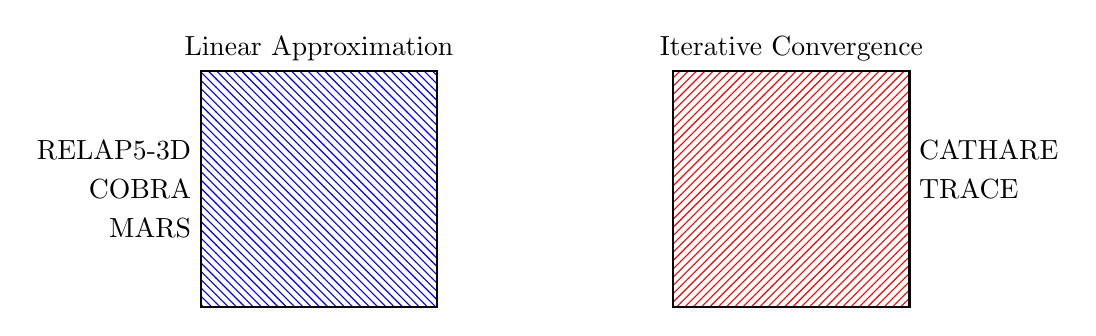
\begin{tikzpicture}
\draw[pattern=north west lines, pattern color=blue] [thick] (-3,0) rectangle (0,3);
\draw (-1.5,3) node[anchor=south] {Linear Approximation};
\draw (-3,2) node[anchor=east] {RELAP5-3D};
\draw (-3,1.5) node[anchor=east] {COBRA};
\draw (-3,1) node[anchor=east] {MARS};
\draw[pattern=north east lines, pattern color=red] [thick] (3,0) rectangle (6,3);
\draw (4.5,3) node[anchor=south] {Iterative Convergence};
\draw (6,2) node[anchor=west] {CATHARE};
\draw (6,1.5) node[anchor=west] {TRACE};
\end{tikzpicture}
}
\end{figure}

\end{frame}
%------------------------------------------------------------------------------
%------------------------------------------------------------------------------
\subsection[Solution Methods]{Solution Methods}
%------------------------------------------------
%------------------------------------------------
\begin{frame}
\frametitle{Semi-Implicit Method}
\textbf{Residual}: $\vec{F}(\vec{x}^{n+1}) = \vec{y}(\vec{x}^{n+1}) - \vec{y}^{n} - \dt{} \vec{E}(\vec{x}^{n+1},\vec{x}^{n})$.

\begin{columns}
\column{\hpw}

\begin{itemize}
\item{Nonlinearities in $\vec{E}(\vec{x}^{n+1},\vec{x}^{n})$}
\item{Single Newton step}
\item{Material Courant limit: $ \Delta t \lesssim \frac{\Delta x}{|u|}$}
\end{itemize}

\column{\hpw}

\begin{algorithmic}
\scriptsize
\Require $\vec{x}^{0}$ and $t^{0}$
\Set $n = 0$
\Loop \; Transient Loop
    \State $t^{n+1} : = t^{n} + \Delta t$
	\Calculate $\vec{F}(\vec{x}^{n})$ and $\vec{J}(\vec{x}^{n})$
	\Calculate $\vec{\delta x} = - \vec{J}^{-1}\cdot\vec{F}$
	\Calculate $\vec{x}^{n+1} = \vec{x}^{n} + \vec{\delta x}$
\EndLoop{\; $n \pluseq 1$} 
\end{algorithmic}
\end{columns}

Problem devolves to an [N x N] matrix for Newton updates of the pressure. 

Used in TRACE, COBRA, RELAP, SPACE, MARS.

\end{frame}
%------------------------------------------------
%------------------------------------------------
\begin{frame}
\frametitle{Semi-Implicit Continuous Liquid Mass and Momentum Equations}

Conservation of continuous liquid mass:
\begin{IEEEeqnarray}{rCl}
V_c \left[ (\alpha_l \rho_l )^{n+1} \right. & - & \left. (\alpha_l \rho_l )^{n} \right] =  -\Delta t \sum_{i \, \in \, N_{f}}\left( \don{\alpha^{n}_{l} \rho^{n}_{l}}^{n}_{d} u^{n+1}_{l} A_{m} \right)_{i} \nonumber \\
&- & \left[ (1-\eta)\Gamma + \Upsilon \right]^{n+1} \nonumber
\end{IEEEeqnarray}

Conservation of continuous liquid momentum:
\begin{IEEEeqnarray}{rcl}
& & \dot{m}_{l}^{n+1} - \dot{m}_{l}^{n} = - \frac{\dt{}}{\dx{}} \left[ \sum_{i \, \in \, N_{c}} \left( \don{\alpha_l \rho_l u_l}_d \ave{u}_{a,l} \tilde{A} \right)^{n}_{i} + \ave{\alpha_{l}}^{n}_{a} \nabla P^{n+1} \right. \nonumber \\
 & & - g\ave{\alpha_l \rho_l}_{a}^{n} + K^{n}_{wl}(\dot{m}_l^{n+1})^2 - K^{n}_{i,gl}(u_{l}^{n+1} - u_{g}^{n+1})^2 \nonumber \\
 & & + \left[(1 - \eta)\dot{\Gamma} u^{'} + \dot{\Upsilon} u^{'}\right]^{n} ] \nonumber
\end{IEEEeqnarray}

\end{frame}
%------------------------------------------------
%------------------------------------------------

%------------------------------------------------------------------------------
%------------------------------------------------------------------------------
%\subsection[Algorithmic Concerns]{Algorithmic Concerns}

%------------------------------------------------------------------------------
%------------------------------------------------------------------------------
\subsection[Domain Coupling]{Domain Coupling}
%------------------------------------------------
%------------------------------------------------
\begin{frame}
\frametitle{Pressure Based Domain Coupling}

\begin{itemize}
\item{Master domain obtains pressure updates in terms of continuity variable flow rates at boundary of slave domains.}
\item{Slave domain contains information about master domain pressures in terms of momentum volume velocities.}
\item{Allows for consistent semi-implicit treatment of entire domain.}
\end{itemize}

\end{frame}
%------------------------------------------------------------------------------
%------------------------------------------------------------------------------
\subsection[Research Objectives]{Research Objectives}

%------------------------------------------------
%------------------------------------------------
\begin{frame}
\frametitle{Research Objectives}

\begin{figure}[t]
\centering
\resizebox{!}{0.7\textheight}{
\tikzsetnextfilename{images/my_diagram_eps}
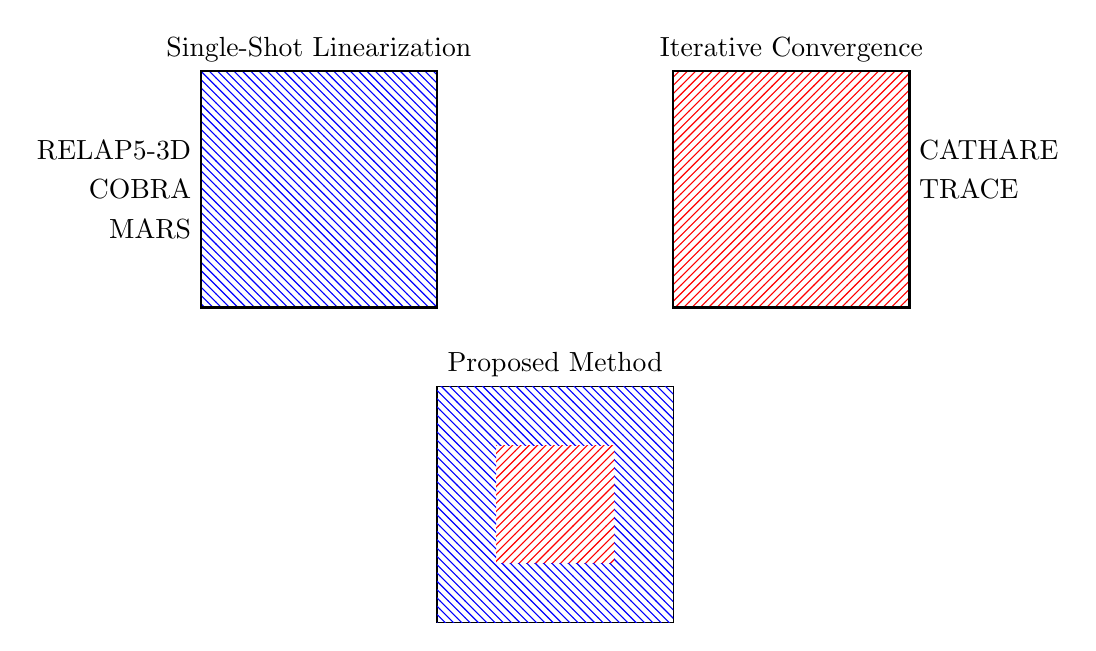
\begin{tikzpicture}
\draw[pattern=north west lines, pattern color=blue] [thick] (-3,0) rectangle (0,3);
\draw (-1.5,3) node[anchor=south] {Single-Shot Linearization};
\draw (-3,2) node[anchor=east] {RELAP5-3D};
\draw (-3,1.5) node[anchor=east] {COBRA};
\draw (-3,1) node[anchor=east] {MARS};
\draw[pattern=north east lines, pattern color=red] [thick] (3,0) rectangle (6,3);
\draw (4.5,3) node[anchor=south] {Iterative Convergence};
\draw (6,2) node[anchor=west] {CATHARE};
\draw (6,1.5) node[anchor=west] {TRACE};
\draw (0,-4) rectangle +(3,3);
\path[pattern=north west lines, pattern color=blue] (0,-4) rectangle +(0.75,3);
\path[pattern=north west lines, pattern color=blue] (2.25,-4) rectangle +(0.75,3);
\path[pattern=north west lines, pattern color=blue] (0.75,-1.75) rectangle +(1.5,0.75);
\path[pattern=north east lines, pattern color=red] (0.75,-3.25) rectangle +(1.5,1.5);
\path[pattern=north west lines, pattern color=blue] (0.75,-4) rectangle +(1.5,0.75);
\draw (1.5,-1) node[anchor=south] {Proposed Method};
\end{tikzpicture}
}
\end{figure}

\end{frame}
%------------------------------------------------
%------------------------------------------------
\subsection[COBRA]{Nonlinear COBRA}
%------------------------------------------------
%------------------------------------------------
\begin{frame}
\frametitle{Nonlinear COBRA}

\begin{itemize}
\item{Original source code assumes that $\vec{x}^{n+1,k} = \vec{x}^{n}$.
    \begin{itemize}
    \item{Temporal derivative terms missing from continuity residuals.}
    \item{Use of $\vec{x}^{n+1,k}$ for $\vec{x}^{n}$.}
    \item{Use of $\vec{x}^{n}$ for $\vec{x}^{n+1,k}$.}
    \end{itemize}
}
\item{Linesearch algorithm with cubic backtracking.}
\item{Quality assurance framework.}
\end{itemize}

\end{frame}
%------------------------------------------------------------------------------
%------------------------------------------------------------------------------
\subsection[Scaling]{Operator Based Scaling}
%------------------------------------------------
%------------------------------------------------
\begin{frame}
\frametitle{Operator-Based Scaling}
Nonlinear residuals have different units:

\begin{IEEEeqnarray}{rcl}
F^{k}_{m,l} & = & V_c \left[ \left(\alpha_l \rho_l \right)^{n+1,k} - \left(\alpha_l \rho_l \right)^{n} \right] + \dt{} \sum_{i\,\in\,N_{f}}\left( \don{\alpha^n_l \rho^n_l}^{n+1,k}_{d} u^{n+1,k}_{l}  A_{m} \right)_{i} \nonumber \\
& + & \left[(1-\eta)\Gamma + \Upsilon \right]^{n+1,k} \nonumber
\end{IEEEeqnarray}

Scaling chosen:

\begin{IEEEeqnarray}{rcl}
S^{k}_{m,l} & = & V_c \abs{\left(\alpha_l \rho_l \right)^{n+1,k} - \left(\alpha_l \rho_l \right)^{n}} + \dt{} \sum_{i\,\in\,N_{f}}\abs{\don{\alpha^n_l \rho^n_l}^{n+1,k}_{d} u^{n+1,k}_l  A_{m}}_{i} \nonumber \\
& + & \abs{(1-\eta)\Gamma}^{n+1,k} + \abs{\Upsilon}^{n+1,k} \nonumber
\end{IEEEeqnarray}

\end{frame}
%------------------------------------------------
%------------------------------------------------
\begin{frame}
\frametitle{Operator-Based Scaling}

\begin{itemize}
\item{$\left( S_{i}^{-1} F_{i} \right)^{k} \approx 1$ when $\vec{x}^{k}$ is a "poor" solution.}
\item{$\left( S_{i}^{-1} F_{i} \right)^{k} \rightarrow 0$ when phase $i$ disappears.}
\item{$0 \leq \abs{ \left( S_{i}^{-1} F_{i} \right)^{k} } \leq 1 $ for all values of $\vec{x}^{k}_i$.}
\end{itemize}

At low volume fractions:
\begin{equation*}
S_{m,l} = \max[1.0, \left(\frac{100 \alpha_{k,\text{min}}}{\alpha_k}\right)^{6} ] S_{m,l}
\end{equation*}

Scaled residual:
\begin{equation*}
\tilde{\vec{F}}(t) = \frac{\vec{F}(t)}{\vec{S}(t)}
\end{equation*}


\end{frame}
%------------------------------------------------------------------------------
%------------------------------------------------------------------------------
\section[Numerical Results]{Numerical Results}
%------------------------------------------------------------------------------
%------------------------------------------------------------------------------
\subsection[Procedures]{Intent and Procedures}
%------------------------------------------------
%------------------------------------------------
\begin{frame}
\frametitle{Numerical Experiments: Purpose}

\begin{itemize}
\item{Test the implementation of the nonlinear solver, and determine its efficacy.}
\item{Test the implementation of the domain decomposition algorithm, and determine its efficacy.}
\item{Determine the impact of not resolving isolated nonlinearities upon the global solution.}
\item{Demonstrate the use of the domain decomposition algorithm in physically relevant scenarios.}
\end{itemize}

\end{frame}
%------------------------------------------------
%------------------------------------------------
\begin{frame}
\frametitle{Numerical Experiments: Procedure}

\begin{itemize}
\item{Timestep size sensitivity studies with the set of \dtmax{} given by
\begin{equation*}
\dtmax{} \in \bigcup^{n_{t}-1}_{i\, = 0} \frac{\dt{}_{0}}{r^{i}_{f}}
\end{equation*}
}
\item{Nonlinear convergence paramters, unless otherwise stated, are \kmax{} = 35, $F_{\text{tol}}$ = \expneg{1.0}{6}, $\delta_{\text{tol}}$ = \expneg{1.0}{8}.}
\end{itemize}

\end{frame}
%------------------------------------------------
%------------------------------------------------
\subsection[Single-Phase and Flashing]{Single-Phase and Flashing Problems}
%------------------------------------------------
%------------------------------------------------
\begin{frame}
\frametitle{Single-Phase and Flashing Problems}
\begin{columns}
\column{0.78\textwidth}

\begin{itemize}
\item{Cross-sectional area: 4 [in$^2$]}
\item{\dx{} is constant: 4 [in]}
\item{IC: Single-Phase: $\alpha_{l} = 1$, @ 200 [psia].}
\item{IC: Flashing: $\alpha_{g}=1$, @ 200 [psia].}
\item{Outlet Conditions $\longleftrightarrow$ Initial Conditions.}
\item{Inlet Conditions: $\alpha_{l}=1$, @ 200 \& 1000 [psia].}
\end{itemize}
\begin{equation*}
\dot{m}(t) = \left\{
\begin{array}{cclrcll}
 0.0           & [\frac{ \lbm{} }{\text{s}}] & , &                & t & \leq 1 & [\text{s}] \\
 0.5 ( t - 1)  & [\frac{ \lbm{} }{\text{s}}] & , & 1\; [\text{s}] < & t & \leq 2 & [\text{s}] \\
 0.5           & [\frac{ \lbm{} }{\text{s}}] & , &                & t & > 2    & [\text{s}]
\end{array}\right.
\end{equation*}

\column{0.22\textwidth}
\begin{figure}[h!t]
\centering
\resizebox{\textwidth}{0.6\textheight}{
\tikzsetnextfilename{images/scaling_test_problem_geometry_pdf}
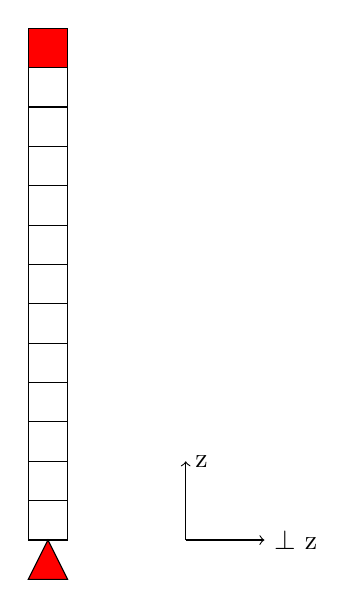
\begin{tikzpicture}
\foreach \x in {1,..., 12} \draw(0, 0.5*\x-0.5) rectangle +(.5,.5);
\filldraw[fill=red] (0, 6) rectangle +(.5,.5); 
\filldraw[fill=red] (0, -0.5) -- (0.25, 0) -- (0.5, -0.5) -- cycle;
\draw[->] (2,0) -- (2, 1) node[anchor=west] {z};
\draw[->] (2,0) -- (3, 0) node[anchor=west] {$\perp$ z};
\end{tikzpicture}
}

\end{figure}
\end{columns}
\end{frame}
%---------
%---------
\begin{frame}
\frametitle{Single-phase solution with \dtmax{} = 1.0 {[s]}}

\begin{figure}[h!t]
\centering
\includegraphics[width=0.94\textwidth]{../plots/single1pt000em0_pdf}
\end{figure}

\end{frame}
%---------
%---------
\begin{frame}
\frametitle{Single-phase solution with \dtmax{} = 1.0E-5 {[s]}}

\begin{figure}[h!t]
\centering
\includegraphics[width=0.94\textwidth]{../plots/single1pt000em5_pdf}
\end{figure}

\end{frame}
%---------
%---------
\begin{frame}
\frametitle{Flashing solution at \dtmax{} = 1.0E-1 {[s]}}

\begin{figure}[h!t]
\centering
\includegraphics[width=0.94\textwidth]{../plots/flashing1pt0000em0_pdf}
\end{figure}

\end{frame}
%---------
%---------
\begin{frame}
\frametitle{Flashing solution at \dtmax{} = 1.0E-5 {[s]}}

\begin{figure}[h!t]
\centering
\includegraphics[width=0.94\textwidth]{../plots/flashing1pt0000em5_pdf}
\end{figure}

\end{frame}
%---------
%---------
\begin{frame}
\frametitle{Legacy solver timestep size insensitive flashing solution}

\begin{figure}[h!t]
\centering
\includegraphics[width=.94\textwidth]{../plots/flashingDtInsensitiveLin_pdf}
\end{figure}

\end{frame}
%---------
%---------
\begin{frame}
\frametitle{Nonlinear solver timestep size insensitive flashing solution}

\begin{figure}[h!t]
\centering
\includegraphics[width=.94\textwidth]{../plots/flashingDtInsensitiveNln_pdf}
\end{figure}

\end{frame}
%---------
%---------
\begin{frame}
\frametitle{Residual of the flashing solution for the legacy solver}

\begin{figure}[h!t]
\centering
\includegraphics[width=0.94\textwidth]{../plots/flashingResidualLin_pdf}
\end{figure}

\end{frame}
%---------
%---------
\begin{frame}
\frametitle{Residual of the flashing solution for the nonlinear solver}

\begin{figure}[h!t]
\centering
\includegraphics[width=0.94\textwidth]{../plots/flashingResidualNln_pdf}
\end{figure}

\end{frame}
%------------------------------------------------
%------------------------------------------------
\subsection[Complex Geometry]{Complex Geometry}
%------------------------------------------------
%------------------------------------------------
\begin{frame}
\frametitle{Complex Geometry}
\begin{columns}
\column{0.7\textwidth}

\begin{itemize}
\item{Model of GE experimental facility.}
\item{3 x 3 rod bundle.}
\item{3 sections.}
\item{18 subchannels.}
\item{56 inter-subchannel flow paths.}
\item{256 different simulations.}
\item{Error = $\displaystyle \sum_{i\,=\,1}^{N_{t}} \abs{P_{\text{lin}}(t^{i}) -P_{k}(t^{i})}$.}
\end{itemize}

\column{0.4\textwidth}

\begin{figure}[h!t]
\centering
\resizebox{\textwidth}{!}{
\begin{center}
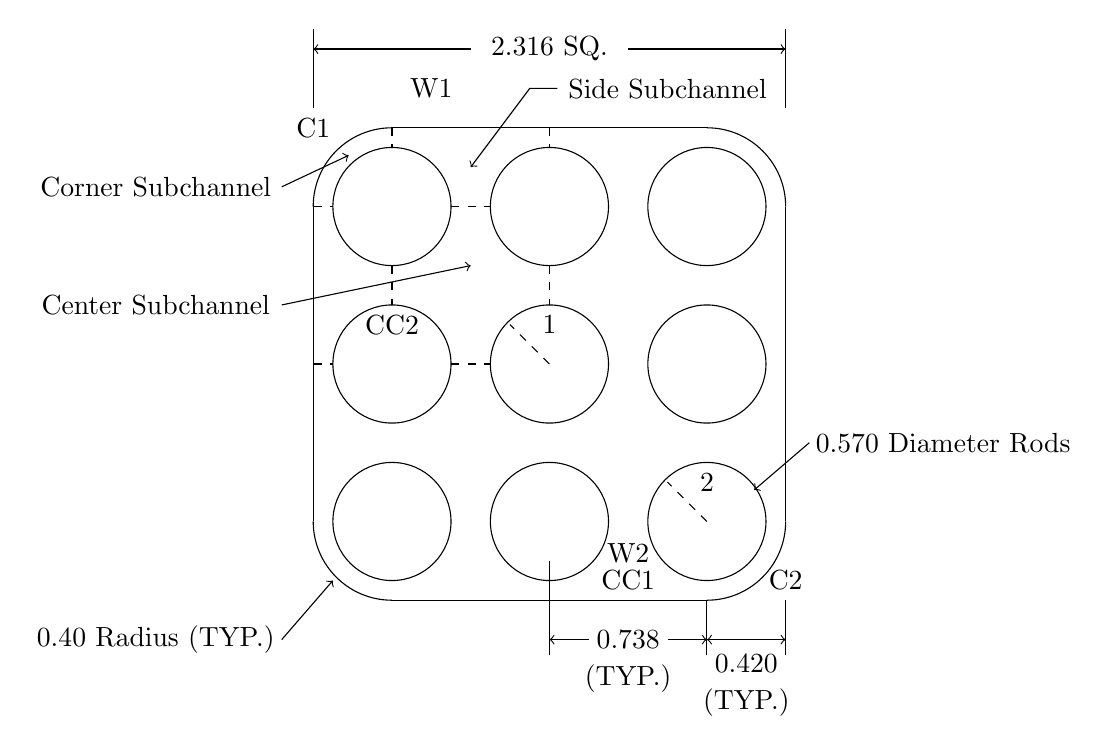
\begin{tikzpicture}

%Rounded corners
\draw (3,2) arc (0:90:1);
\draw (-2,3) arc (90:180:1);
\draw (-3,-2) arc (180:270:1);
\draw (2,-3) arc (270:360:1);

%Grid of circles
\draw (0,0) circle (0.75);
\draw (0,2) circle (0.75);
\draw (0,-2) circle (0.75);
\draw (2,0) circle (0.75);
\draw (2,2) circle (0.75);
\draw (2,-2) circle (0.75);
\draw (-2,0) circle (0.75);
\draw (-2,2) circle (0.75);
\draw (-2,-2) circle (0.75);

%Box
\draw (-3,-2) -- (-3,2);
\draw (3,-2) -- (3,2);
\draw (2,-3) -- (-2,-3);
\draw (-2,3) -- (2,3);

%Misc lines
\draw [dashed] (-2,3) -- (-2,2.75);
\draw [dashed] (0,3) -- (0,2.75);
\draw [dashed] (-2,1.25) -- (-2,0.75);
\draw [dashed] (0,1.25) -- (0,0.75);
\draw [dashed] (-3,2) -- (-2.75,2);
\draw [dashed] (-3,0) -- (-2.75,0);
\draw [dashed] (-1.25,2) -- (-0.75,2);
\draw [dashed] (-1.25,0) -- (-0.75,0);

\draw [dashed] (0,0) -- (-0.5,0.5);
\draw [dashed] (2,-2) -- (1.5,-1.5);

%Misc arrows and labels
\draw [<-] (-3,4) -- (-1,4);
\draw [->] (1,4) -- (3,4);
\draw (-3,4.25) -- (-3,3.25);
\draw (3,4.25) -- (3,3.25);
\draw (0,4) node {2.316 SQ.};

\draw [<-] (0,-3.5) -- (0.5,-3.5);
\draw [->] (1.5,-3.5) -- (2,-3.5);
\draw (2,-3.7) -- (2,-3);
\draw (0,-3.7) -- (0,-2.5);
\draw (1,-3.5) node {0.738};
\draw (1,-4) node {(TYP.)};

\draw [<->] (2,-3.5) -- (3,-3.5);
\draw (3,-3.7) -- (3,-3);
\draw (2.5,-3.8) node {0.420};
\draw (2.5,-4.3) node {(TYP.)};

\draw [->] (-3.4,2.25) -- (-2.55,2.65);
\draw (-5,2.25) node {Corner Subchannel};

\draw [->] (-3.4,0.75) -- (-1,1.25);
\draw (-5,0.75) node {Center Subchannel};

\draw [->] (0.1,3.5) -- (-0.25,3.5) -- (-1,2.5);
\draw (1.5,3.5) node {Side Subchannel};

\draw [->] (-3.4,-3.5) -- (-2.75,-2.75);
\draw (-5,-3.5) node {0.40 Radius (TYP.)};

\draw [->] (3.3,-1) -- (2.6,-1.6);
\draw (5,-1) node {0.570 Diameter Rods};

\draw (-3,3) node {C1};
\draw (-1.5,3.5) node {W1};
\draw (1,-2.75) node {CC1};

\draw (3,-2.75) node {C2};
\draw (1,-2.4) node {W2};
\draw (-2,0.5) node {CC2};

\draw (0,0.5) node {1};
\draw (2,-1.5) node {2};

\end{tikzpicture}
\end{center}
\caption{Position of pressure taps for setting isokinetic conditions. Note splitter positions for the various subchannels.}
\label{fig:position_of_pressure taps}
}
\end{figure}

\end{columns}
\end{frame}
%---------
%---------
\begin{frame}
\frametitle{Error in Complex Geometry Problem}

\begin{figure}[h!t]
\centering
\includegraphics[width=0.94\textwidth]{../plots/complexBar_pdf}
\end{figure}

\end{frame}
%------------------------------------------------
%------------------------------------------------
\subsection[Valve Problem]{Valve Problem}
%------------------------------------------------
%------------------------------------------------
\begin{frame}
\frametitle{Valve Problem}

\begin{itemize}
\item{Four 40 [in] subchannels: $A_{c} = 16$ [in$^{2}$], \dx{} = 4 [in].}
\item{Conditions:
	\begin{itemize}
	\item{Initial $\rightarrow$ $\alpha_{l} = 1$ @ 800 [psia].}
	\item{Inlet $\rightarrow$ $\alpha_{l} = 1$ @ 818 [psia].}
	\item{Outlet $\rightarrow$ $\alpha_{l} = 1$ @ 800 [psia].}
	\end{itemize}
}
\item{Obstructions @ 15 [in]:
\begin{itemize}
	\item{Subchannel 1 $\rightarrow$ K = $\infty$ [-].}
	\item{Subchannel 2 $\rightarrow$ K = 40 [-].}
	\item{Subchannel 3 $\rightarrow$ K = 160 [-].}
	\item{Subchannel 4 $\rightarrow$ K(t) $\rightarrow K(t) = \frac{K_{o}}{{A(t)_r}^2}$, $K_{o} = 10$ [-].}
\end{itemize}
}
\item{No connections between channels.}
\end{itemize}

\end{frame}
%---------
%---------
\begin{frame}
\frametitle{Time Dependent Area}

\begin{figure}[h!t]
\centering
\includegraphics[width=0.94\textwidth]{../plots/valveTransientArea_pdf}
\end{figure}

\end{frame}
%---------
%---------
\begin{frame}
\frametitle{Linear Solver's Solutions}

\begin{figure}[h!t]
\centering
\includegraphics[width=0.94\textwidth]{../plots/valveLinSols_pdf}
\end{figure}

\end{frame}
%---------
%---------
\begin{frame}
\frametitle{Nonlinear and Domain Decomposition Solver's Solutions}

\begin{figure}[h!t]
\centering
\includegraphics[width=0.94\textwidth]{../plots/valveNlnSols_pdf}
\end{figure}

\end{frame}
%---------
%---------
\begin{frame}
\frametitle{Run Time Comparison}

\begin{figure}[h!t]
\centering
\includegraphics[width=0.94\textwidth]{../plots/valveRunTime_pdf}
\end{figure}

\end{frame}
%------------------------------------------------
%------------------------------------------------
\subsection[Filling Problem]{Filling Problem}
%------------------------------------------------
%------------------------------------------------
\begin{frame}
\frametitle{Filling Problem}

\begin{itemize}
\item{2 Subchannels}
\item{Dimensions: $A_{c}$ = 36 [in$^2$]; \dx{} = 4 [in].}
\item{IC: Single-Phase: $\alpha_{g} = 1$, @ 14.7 [psia].}
\item{Outlet $\longleftrightarrow$ Initial Conditions.}
\item{Inlet $\rightarrow$ $\alpha_{l}=1$, @ 14.7 [psia].}
\end{itemize}
\begin{equation*}
P(t, h(t))= 
 \left\{
\begin{array}{cclrcll}
P_o & [ \text{psia} ] & , & 0\; [\text{s}] < & t & \leq t^{*}(h) & [\text{s}] \\
P_o + g \frac{ h(t) - h }{ v_{l} } & [ \text{psia} ] & , &  & t & > t^{*}(h) & [\text{s}]
\end{array}\right.
\end{equation*}

\end{frame}
%---------
%---------
\begin{frame}
\frametitle{Analytic Solution}

\begin{figure}[h!t]
\centering
\includegraphics[width=0.94\textwidth]{../plots/vmpAnalytic_pdf}
\end{figure}

\end{frame}
%---------
%---------
\begin{frame}
\frametitle{Linear Solution}

\begin{figure}[h!t]
\centering
\includegraphics[width=0.94\textwidth]{../plots/vmpLinear1em1_pdf}
\end{figure}

\end{frame}
%---------
%---------
\begin{frame}
\frametitle{Linear \dtmax{}}

\begin{figure}[h!t]
\centering
\includegraphics[width=0.94\textwidth]{../plots/vmpDeltaTLin1em1_pdf}
\end{figure}

\end{frame}
%---------
%---------
\begin{frame}
\frametitle{Nonlinear Solution}

\begin{figure}[h!t]
\centering
\includegraphics[width=0.94\textwidth]{../plots/vmpNLN1em1_pdf}
\end{figure}

\end{frame}
%---------
%---------
\begin{frame}
\frametitle{Nonlinear \dtmax{}}

\begin{figure}[h!t]
\centering
\includegraphics[width=0.94\textwidth]{../plots/vmpDeltaTNln1em1_pdf}
\end{figure}

\end{frame}
%---------
%---------
\begin{frame}
\frametitle{Bottom Section in Nonlinear Domain}

\begin{figure}[h!t]
\centering
\includegraphics[width=0.94\textwidth]{../plots/vmpBotNln1em1_pdf}
\end{figure}

\end{frame}
%---------
%---------
\begin{frame}
\frametitle{Top Section in Nonlinear Domain}

\begin{figure}[h!t]
\centering
\includegraphics[width=0.94\textwidth]{../plots/vmpTopNln1em1_pdf}
\end{figure}

\end{frame}
%------------------------------------------------
%------------------------------------------------
\subsection[Post-blowdown Refill Problem]{Post-blowdown Refill Problem}
%------------------------------------------------
%------------------------------------------------
\begin{frame}
\frametitle{Post-blowdown Refill Problem}
\begin{columns}
\column{0.80\textwidth}
\begin{itemize}
\item{Simplified model of PWR reactor pressure vessel.}
\item{Simulation starts after blow-down stage of LOCA.}
\item{Conditions:
\begin{itemize}
\item{Section 1 $\rightarrow$ $\alpha_{l} = 1$.}
\item{Downcomer: Mix of air and steam.}
\item{Core: Steam.}
\item{Containment @ A}
\item{Safety Injection @ B @ 25 $\displaystyle \left[ \frac{\lbm{}}{\text{s}} \right]$ @ 20 [s].}
\item{Steam Generation @ Points C \& D @ 25 [s].}
\end{itemize}
}
\end{itemize}


\column{0.20\textwidth}
\begin{figure}[h!t]
\centering
\resizebox{!}{0.65\textheight}{\tikzsetnextfilename{images/refillSimpleModel_pdf}
{
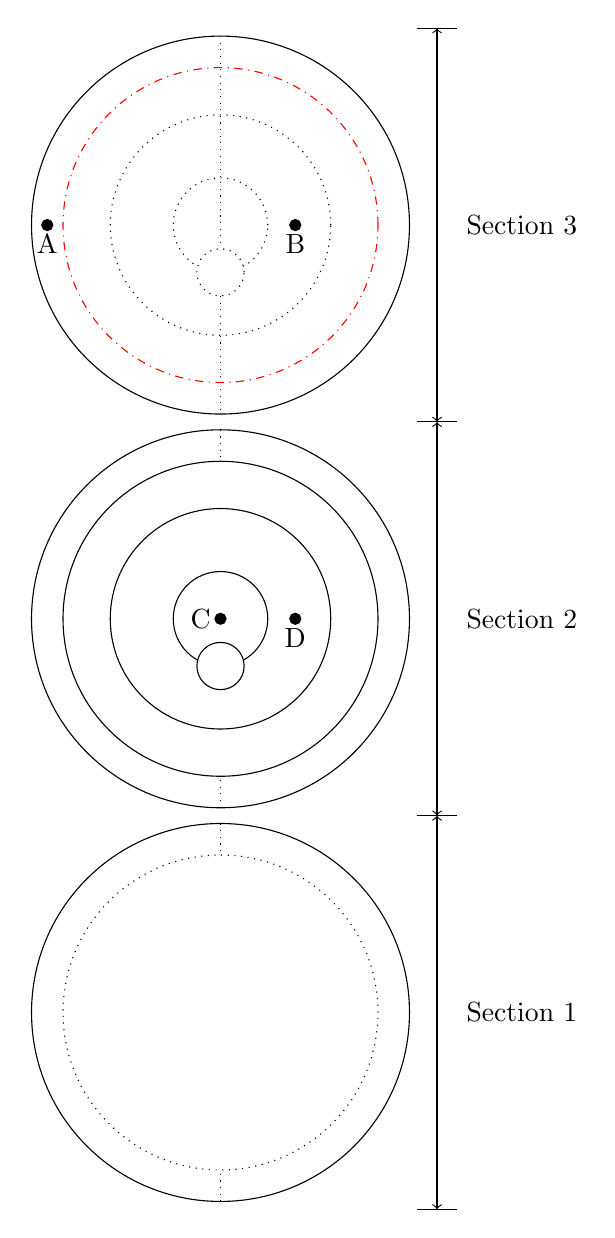
\begin{tikzpicture}

%Section 3 Flow Pattern
\draw [dotted] (0.0, 11.9) -- (0, 9.2);
\draw [dotted] (0.0, 8.6) -- (0, 7.1);
\draw [dotted] (0.0, 9.5) circle (0.6);
\draw [dotted] (0.0, 9.5) circle (1.4);
\draw [dashdotted, color=red]  (0.0, 9.5) circle (2.0);
\draw [solid]  (0.0, 9.5) circle (2.4);
\filldraw [dotted, fill=white, draw=black] (0.0, 8.9) circle (0.3);
\filldraw [black] ( 0.95, 9.5) circle (2pt) node[anchor=north]{B};
\filldraw [black] (-2.20, 9.5) circle (2pt) node[anchor=north]{A};	

%Section 2 Flow Pattern
\draw [solid] (0.0, 4.5) circle (0.6);
\draw [solid] (0.0, 4.5) circle (1.4);
\draw [solid] (0.0, 4.5) circle (2.0);
\draw [solid] (0.0, 4.5) circle (2.4);
\filldraw [fill=white, draw=black] (0.0, 3.9) circle (0.3);
\draw [dotted] (0.0, 6.9) -- (0.0, 6.5);
\draw [dotted] (0.0, 2.1) -- (0.0, 2.5);
\filldraw [black] (0.0, 4.5) circle (2pt) node[anchor=east]{C};	
\filldraw [black] ( 0.95, 4.5) circle (2pt) node[anchor=north]{D};

%Section 1 Flow Pattern
\draw [solid]  (0.0, -0.5) circle (2.4);
\draw [dotted] (0.0, -0.5) circle (2.0);
\draw [dotted] (0.0,  1.9) -- (0.0,  1.5);
\draw [dotted] (0.0, -2.9) -- (0.0, -2.5);

%Arrows & Labels
\draw (2.5,12) -- (3,12);
\draw [<->] (2.75,12) -- (2.75,7);
\draw (2.5,7) -- (3,7);
\draw [<->] (2.75,7) -- (2.75,2);
\draw (2.5,2) -- (3,2);
\draw [<->] (2.75,2) -- (2.75,-3);
\draw (2.5,-3) -- (3,-3);
\foreach \y/\ytext in {-0.5/Section 1,4.5/Section 2,9.5/Section 3}
	\draw (3,\y) node [anchor=west] {\ytext};

%Extras
\end{tikzpicture}
}}
\end{figure}
\end{columns}

\end{frame}
%---------
%---------
\begin{frame}
\frametitle{Steam Generation Rate}

\begin{figure}[h!t]
\centering
\includegraphics[width=0.94\textwidth]{../plots/refillSteamRates_pdf}
\end{figure}

\end{frame}
%---------
%---------
\begin{frame}
\frametitle{Downcomer and Core Effective Volume Fractions}

\begin{figure}[h!t]
\centering
\includegraphics[width=0.94\textwidth]{../plots/refillCoreVolFracDom_pdf}
\end{figure}

\end{frame}
%---------
%---------
\begin{frame}
\frametitle{Linear Solver's Net Condensation}

\begin{figure}[h!t]
\centering
\includegraphics[width=0.94\textwidth]{../plots/refillGammaLin_pdf}
\end{figure}

\end{frame}%---------
%---------
\begin{frame}
\frametitle{Nonlinear Solver's Net Condensation}

\begin{figure}[h!t]
\centering
\includegraphics[width=0.94\textwidth]{../plots/refillGammaNln_pdf}
\end{figure}

\end{frame}
%---------
%---------
\begin{frame}
\frametitle{Dual-Domain Solver's Net Condensation}

\begin{figure}[h!t]
\centering
\includegraphics[width=0.94\textwidth]{../plots/refillGammaDom_pdf}
\end{figure}

\end{frame}
%---------
%---------
\begin{frame}
\frametitle{Maximum Condensation v. \dtmax{}}

\begin{figure}[h!t]
\centering
\includegraphics[width=0.94\textwidth]{../plots/refillMaxGamma_pdf}
\end{figure}

\end{frame}
%---------
%---------
\begin{frame}
\frametitle{Run Time Ratios}

\begin{figure}[h!t]
\centering
\includegraphics[width=0.94\textwidth]{../plots/refillRunTimeRatios_pdf}
\end{figure}

\end{frame}
%------------------------------------------------------------------------------
%------------------------------------------------------------------------------
\section[Conclusions]{Conclusions}
\subsection[Conclusions]{Conclusions}
\begin{frame}
\frametitle{Summary}

\begin{itemize}
\item{Methods that resolve nonlinearities during a timestep allow for a more timestep size insensitive solution at larger \dtmax{} than methods that do not.}
\item{A timestep size insensitive solution produced by a linearized approximation may be different than one produced by a nonlinearly convergent solver.}
\item{Not resolving localized nonlinearities can degrade the accuracy of the solution globally.}
\item{By using the domain decomposition algorithm to resolve localized nonlinearities, a simulation can achieve the accuracy and consistency of a fully nonlinear solver without its associated computational costs.}
\end{itemize}

\end{frame}
%------------------------------------------------------------------------------
%------------------------------------------------------------------------------
\subsection[Future Work]{Future Work}
\begin{frame}
\frametitle{Future Work}

\begin{itemize}
\item{Development of a way to adaptively determine when and where additional nonlinear iterates would be advantageous.}
\item{Investigate the computational costs of the general algorithm to determine when it would be more advantageous to include the entire domain in the nonlinear domain than it would be to use the domain decomposition algorithm.}
\item{Investigate the interaction between the nonlinear hydrodynamic solver and the explicit fluid-solid heat transfer.}
\item{Investigate impact of switching governing equations upon nonlinear convergence.}
\end{itemize}

\end{frame}
%------------------------------------------------
%------------------------------------------------
%------------------------------------------------------------------------------
%------------------------------------------------------------------------------
\section*{}
%------------------------------------------------
%------------------------------------------------
\begin{frame}
\frametitle{Acknowledgments}

This research was performed under appointment to the Rickover Fellowship Program in Nuclear Engineering sponsored by Naval Reactors Division of the U.S. Department of Energy.

\end{frame}
%------------------------------------------------
%------------------------------------------------
%\begin{frame}
%\frametitle{Conservation of Mass}
%
%\begin{IEEEeqnarray}{rCl}
%\frac{\partial \left(\alpha_g \rho_{n}\right) }{\partial t } + \nabla \cdot \left( \alpha_g \rho_{n} \vec{u}_g \right) & = & s_{m,n} \nonumber \\
%\frac{\partial \left(\alpha_g \rho_v \right)}{\partial t } + \nabla \cdot \left( \alpha_g \rho_v \vec{u}_g \right)         & = & \Gamma^{'''} + s_{m,v} \nonumber \\
%\frac{\partial \left(\alpha_l \rho_l \right)}{\partial t } + \nabla \cdot \left( \alpha_l \rho_l \vec{u}_l \right)         & = & -(1-\eta)\Gamma^{'''} - S^{'''} + s_{m,l} \nonumber \\
%\frac{\partial \left(\alpha_e \rho_l \right)}{\partial t } + \nabla \cdot \left( \alpha_e \rho_l \vec{u}_e \right)         & = & -\eta\Gamma^{'''} + S^{'''}+ s_{m,e} \nonumber
%\end{IEEEeqnarray}
%
%\end{frame}
%%------------------------------------------------
%%------------------------------------------------
%\begin{frame}
%\frametitle{Conservation of Momentum}
%
%\begin{IEEEeqnarray}{rCl}
%\frac{\partial \left( \alpha_l \rho_l \vec{u}_l \right )}{\partial t } + \nabla \cdot \left( \alpha_l \rho_l \vec{u}_l \vec{u}_l \right) & = & \nonumber \\
% -\alpha_l \nabla P + \alpha_l \rho_l \vec{g} - \vec{\tau}^{'}_{w,l} + \vec{\tau}^{'}_{i,gl} - (1 - \eta)\Gamma^{'''}\vec{u}^{'} - S^{'''}\vec{u}^{'} + s_{p,l} & & \nonumber \\
%\frac{\partial \left( \alpha_g \rho_g \vec{u}_g \right) }{\partial t } + \nabla \cdot \left( \alpha_g \rho_g \vec{u}_g \vec{u}_g \right) & = & \nonumber \\
% -\alpha_g \nabla P + \alpha_g \rho_g \vec{g} - \vec{\tau}^{'}_{w,g} - \vec{\tau}^{'}_{i,gl} - \vec{\tau}^{'}_{i,ge} + \Gamma^{'''}\vec{u}^{'} + s_{p,g} & & \nonumber \\
%\frac{\partial \left( \alpha_e \rho_l \vec{u}_e \right) }{\partial t } + \nabla \cdot \left( \alpha_e \rho_l \vec{u}_e \vec{u}_e \right) & = & \nonumber \\
% -\alpha_e \nabla P + \alpha_e \rho_l \vec{g} - \vec{\tau}^{'}_{w,l} + \vec{\tau}^{'}_{i,ge} - \eta \Gamma^{'''}\vec{u}^{'} + S^{'''}\vec{u}^{'} + s_{p,l} & & \nonumber
%\end{IEEEeqnarray}
%
%\end{frame}
%%------------------------------------------------
%%------------------------------------------------
%\begin{frame}
%\frametitle{Conservation of Energy}
%
%\begin{IEEEeqnarray}{rCl}
%\frac{\partial \left( \alpha_g \{\rho_g h_g\} \right)}{\partial t } + \nabla \cdot \left(  \alpha_g \{\rho_g h_g\} \vec{u}_g \right) & =& \nonumber \\
%\Gamma^{'''} h^{'}_v + q^{'''}_{i,v} + q^{'''}_{n,l}  + q^{'''}_{w,g} + \alpha_g\frac{\partial P}{\partial t} + s_{e,g}  & & \nonumber \\
%\frac{\partial \left( (1 - \alpha_g) \rho_l h_l \right) }{\partial t } + \nabla \cdot \left( \alpha_l \rho_l h_l \vec{u}_l \right) + \nabla \cdot \left( \alpha_e \rho_l h_l \vec{u}_e \right)& = & \nonumber \\
%-\Gamma^{'''} h^{'}_l +  q^{'''}_{i,l} - q^{'''}_{n,l}  + q^{'''}_{w,l} + (1 - \alpha_g) \frac{\partial P}{\partial t} + s_{e,l}  & & \nonumber
%\end{IEEEeqnarray}
%
%\begin{equation*}
%\label{eqn:gaseous_enthalpy}
%\alpha_g \{\rho_g h_g\} = \alpha_g \rho_v h_v + \alpha_g \rho_n h_n
%\end{equation*}
%
%\end{frame}
%%------------------------------------------------
%%------------------------------------------------
%\begin{frame}
%\frametitle{Methods}
%\begin{itemize}
%\item{Fully Explicit Method
%\begin{itemize}
%\item{Lowest computational cost per timestep}
%\item{Subject to sonic CFL limit: $ \dt{} \lesssim \frac{\dx{}}{|u|+|c|}$}
%\end{itemize}
%}
%\item{Fully Implicit Method
%\begin{itemize}
%\item{Highest computational cost per timestep.}
%\item{Not subject to CFL limit.}
%\item{Nonlinearly convergent}
%\item{CATHARE (Barre and Bernard, 1990)}
%\end{itemize}
%}
%\item{Semi-Implicit Method (Liles and Reed, 1978)
%\begin{itemize}
%\item{Single Newton step}
%\item{Subject to material Courant limit: $ \dt{} \lesssim \frac{\dx{}}{|u|}$}
%\item{RELAP, TRACE, COBRA, MARS, SPACE} 
%\end{itemize}
%}
%\end{itemize}
%\end{frame}
%%------------------------------------------------
%%------------------------------------------------
%\begin{frame}
%\frametitle{Methods}
%\begin{itemize}
%\item{Stability-Enhancing Two-Step Method (SETS) (Mahaffy, 1982)
%\begin{itemize}
%\item{Multistage method}
%\item{Nonlinearly convergent}
%\item{Capable of exceeding material Courant limit}
%\item{TRAC-M/Fortran 90, TRACE}
%\end{itemize}
%}
%\item{Nearly Implicit Method (Trapp and Riemke, 1986)
%\begin{itemize}
%\item{Derivative of SETS method}
%\item{Multistage method}
%\item{Single Newton step}
%\item{Capable of exceeding material Courant limit}
%\item{RELAP}
%\end{itemize}
%}
%\end{itemize}
%
%\end{frame}
%%------------------------------------------------
%%------------------------------------------------
%\begin{frame}
%\frametitle{Fully Explicit Method}
%Residual: $\vec{F}(\vec{x}^{n+1}) = \vec{y}(\vec{x}^{n+1}) - \vec{y}^{n} - \dt{} \vec{E}(\vec{x}^{n})$.
%\begin{columns}
%\column{0.45\textwidth}
%\begin{itemize}
%\item{Lowest per timestep computational cost.}
%\item{Nonlinearities in the new-time conserved quantities.}
%\item{Sonic Courant limit: $ \Delta t \lesssim \frac{\Delta x}{|u|+|c|}$}
%\end{itemize}
%
%\column{0.55\textwidth}
%\begin{algorithmic}
%\scriptsize
%\Require $\vec{x}^{0}$ and $t^{0}$
%\Set $n = 0$
%\Loop \; Take a Time Step
%    \Set $t^{n+1} : = t^{n} + \Delta t$
%    \Calculate $\vec{F}(\vec{x}^n)$ and $\vec{J}(\vec{x}^n)$
%    \Calculate $\vec{\delta x} = -\vec{J}^{-1}\vec{F}$
%    \Calculate $\vec{x}^{n+1} = \vec{x}^{n} + \vec{\delta x}$ 
%\EndLoop{\;$n = n+1$}
%\end{algorithmic}
%
%\end{columns}
%
%\end{frame}
%%------------------------------------------------
%%------------------------------------------------
%\begin{frame}
%\frametitle{Fully Implicit Method}
%
%Residual: $\vec{F}(\vec{x}^{n+1}) = \vec{y}(\vec{x}^{n+1}) - \vec{y}^{n} - \dt{} \vec{E}(\vec{x}^{n+1})$.
%
%\begin{columns}
%\column{0.45\textwidth}
%
%\begin{itemize}
%\item{Highest per timestep computational cost.}
%\item{Nonlinearities in $\vec{E}(\vec{x}^{*})$.}
%\item{No Courant limit.}
%\item{CATHARE}
%\end{itemize}
%
%\column{0.55\textwidth}
%
%\begin{algorithmic}
%\scriptsize
%\Require $\vec{x}^{0}$ and $t^{0}$
%\Set $n = 0$
%\Loop \; Transient Loop
%    \Set $t^{n+1} : = t^{n} + \Delta t$
%    \Set $k = 0$
%    \Set $\vec{x}^{k} = \vec{x}^{n}$
%    \Loop \; Newton Loop
%		\Calculate $\vec{F}(\vec{x}^{k})$ and $\vec{J}(\vec{x}^{k})$
%		\Calculate $\vec{\delta x}^k = - \vec{J}^{-1}\cdot\vec{F}$
%		\BlackBox Calculate $\vec{x}^{k+1}$
%		\BlackBox Terminate Loop
%	\EndLoop{\;$k = k + 1$} 	
%\EndLoop{\;$n = n + 1$}
%\end{algorithmic}
%
%\end{columns}
%\end{frame}
%%------------------------------------------------
%%------------------------------------------------
%\begin{frame}
%\frametitle{Stability-Enhancing Two-Step Method}
%
%\begin{columns}
%\column{0.45\textwidth}
%
%\begin{itemize}
%\item{Developed to overcome material Courant limit of the semi-implicit method.}
%\item{Multistage approximation to $\vec{E}(\vec{x}^{*})$.}
%\item{Courant limit above the material Courant limit but not unbounded.}
%\item{TRACE}
%\end{itemize}
%
%\column{0.5\textwidth}
%\begin{algorithmic}
%\scriptsize
%\Require $\vec{x}^{0}$ and $t^{0}$
%\Set $n = 0$
%\Loop \; Transient Loop
%    \State $t^{n+1} : = t^{n} + \Delta t$
%	\Calculate $\vec{F}_1$ and $\vec{J}_1$
%	\Calculate $\vec{u}^{*}$ from $\vec{\delta u}^{*} = -\vec{J}^{-1}_1\vec{F}_1$
%	\Loop \; Newton Loop
%		\Calculate $\vec{F}_2$ and $\vec{J}_2$
%		\Calculate $\vec{\delta x} = - \vec{J}_2^{-1}\vec{F}_2$
%		\Calculate $\vec{x}^{n+1} = \vec{x}^{n} + \vec{\delta x}$
%	\EndLoop
%	\Calculate $\vec{x}^{n+1}$ from $\vec{F}_3$.
%\EndLoop{\; $n = n + 1$} 
%\end{algorithmic}
%
%\end{columns}
%\end{frame}
%%------------------------------------------------
%%------------------------------------------------
%\begin{frame}
%\frametitle{Nearly-Implicit Method}
%
%\begin{columns}
%\column{0.45\textwidth}
%
%\begin{itemize}
%\item{Derivative of SETS method.}
%\item{Developed to overcome material Courant limit of the semi-implicit method.}
%\item{Three-stage approximation to $\vec{E}(\vec{x}^{*})$.}
%\item{Courant limit above the material Courant limit but not unbounded.}
%\item{Two-stage variant used in RELAP5-3D}
%\end{itemize}
%
%\column{0.5\textwidth}
%\begin{algorithmic}
%\scriptsize
%\Require $\vec{x}^{0}$ and $t^{0}$
%\Set $n = 0$
%\Loop \; Transient Loop
%    \State $t^{n+1} : = t^{n} + \Delta t$
%	\Calculate $\vec{F}_1$ and $\vec{J}_1$
%	\Calculate $\vec{\delta x}^{*} = -\vec{J}^{-1}_1\vec{F}_1$
%	\Calculate $\vec{c}^{*}$ and $\vec{u}^{n+1}$
%	\Calculate $\vec{F}_2$
%	\Calculate $\vec{c}^{**}$ from $\vec{F}_2$
%	\Calculate $\vec{c}^{n+1}$ from $\vec{F}_3$.
%\EndLoop{\; $n = n + 1$}
%\end{algorithmic}
%
%\end{columns}
%
%\end{frame}
%%------------------------------------------------
%%------------------------------------------------
%\begin{frame}
%\frametitle{Semi-Implicit Equation Ordering}
%
%\begin{itemize}
%\item{Continuity Volumes
%\begin{enumerate}
%\item{Conservation of the \ncg{} field mass.}
%\item{Conservation of the vapor field mass.}
%\item{Conservation of the gaseous phase energy.}
%\item{Conservation of the liquid phase energy.}
%\item{Conservation of the entrained liquid field mass.}
%\item{Conservation of the continuous liquid field mass.}
%\end{enumerate}
%}
%\item{Momentum Volumes
%\begin{enumerate}
%\item{Conservation of the continuous liquid field momentum.}
%\item{Conservation of the gaseous phase momentum.}
%\item{Conservation of the entrained liquid field momentum.}
%\end{enumerate}
%}
%\end{itemize}
%
%\end{frame}
%%------------------------------------------------
%%------------------------------------------------
%\begin{frame}
%\frametitle{Semi-Implicit Method Solution Algorithm}
%
%Example: 3 continuity volumes and 3 momentum volumes.
%
%\begin{equation*}
%\begin{bmatrix} 
%\vec{J}_{m_1} & \vec{J}_{m_1,c_1} & \vec{0} & \vec{0} & \vec{0} & \vec{0}\\
%\vec{J}_{c_1,m_1} & \vec{J}_{c_1} & \vec{J}_{c_1,m_2} & \vec{0} & \vec{0} & \vec{0} \\
%\vec{0} & \vec{J}_{m_2,c_1} & \vec{J}_{m_2} & \vec{J}_{m_2,c_2} & \vec{0} & \vec{0} \\
%\vec{0} & \vec{0} & \vec{J}_{c_2,m_2} & \vec{J}_{c_2} & \vec{J}_{c_2,m_3} & \vec{0} \\
%\vec{0} & \vec{0} & \vec{0} & \vec{J}_{m_3,c_2} & \vec{J}_{m_3} & \vec{J}_{m_3,c_3} \\ 
%\vec{0} & \vec{0} & \vec{0} & \vec{0} & \vec{J}_{c_3,m_3} & \vec{J}_{c_3}  
%\end{bmatrix} \begin{bmatrix}
%\vec{\delta m}_{1} \\ \vec{\delta c}_{1} \\
%\vec{\delta m}_{2} \\ \vec{\delta c}_{2} \\
%\vec{\delta m}_{3} \\ \vec{\delta c}_{3}
%\end{bmatrix}  = -\begin{bmatrix}
%\vec{F}_{m_1} \\ \vec{F}_{c_1} \\
%\vec{F}_{m_2} \\ \vec{F}_{c_2} \\
%\vec{F}_{m_3} \\ \vec{F}_{c_3} \end{bmatrix}
%\end{equation*}
%
%\end{frame}
%%------------------------------------------------
%%------------------------------------------------
%\begin{frame}
%\frametitle{Semi-Implicit Method Solution Algorithm}
%
%Multiply momentum equations by their inverse Jacobians.
%
%\begin{equation*}
%\begin{bmatrix} 
%\vec{I} & \frac{\partial \vec{m}_1}{\partial P_1} & \vec{0} & \vec{0} & \vec{0} & \vec{0}\\
%\vec{J}_{c_1,m_1} & \vec{J}_{c_1} & \vec{J}_{c_1,m_2} & \vec{0} & \vec{0} & \vec{0} \\
%\vec{0} & \frac{\partial \vec{m}_2}{\partial P_1} & \vec{I} & \frac{\partial \vec{m}_2}{\partial P_2} & \vec{0} & \vec{0} \\
%\vec{0} & \vec{0} & \vec{J}_{c_2,m_2} & \vec{J}_{c_2} & \vec{J}_{c_2,m_3} & \vec{0} \\
%\vec{0} & \vec{0} & \vec{0} & \frac{\partial \vec{m}_{3}}{\partial P_2} & \vec{I} & \frac{\partial \vec{m}_{3}}{\partial P_3} \\ 
%\vec{0} & \vec{0} & \vec{0} & \vec{0} & \vec{J}_{c_3,m_3} & \vec{J}_{c_3}  
%\end{bmatrix} \begin{bmatrix}
%\vec{\delta m}_{1} \\ \vec{\delta c}_{1} \\
%\vec{\delta m}_{2} \\ \vec{\delta c}_{2} \\
%\vec{\delta m}_{3} \\ \vec{\delta c}_{3}
%\end{bmatrix}  = -\begin{bmatrix}
%\vec{J}^{-1}_{m_1}\vec{F}_{m_1} \\ \vec{F}_{c_1} \\
%\vec{J}^{-1}_{m_2}\vec{F}_{m_2} \\ \vec{F}_{c_2} \\
%\vec{J}^{-1}_{m_3}\vec{F}_{m_3} \\ \vec{F}_{c_3} \end{bmatrix}
%\end{equation*}
%
%\begin{equation*}
%\frac{\partial \vec{m}_k}{\partial P_j} = \vec{J}^{-1}_{m_k}\vec{J}_{m_k,c_j}
%\end{equation*}
%
%\end{frame}
%%------------------------------------------------
%%------------------------------------------------
%\begin{frame}
%\frametitle{Semi-Implicit Method Solution Algorithm}
%
%\begin{equation*}
%\resizebox{1.0\textwidth}{!}{$
%\begin{bmatrix} 
%\vec{J}_{c_1} - \vec{J}_{c_1,m_1}\frac{\partial \vec{m}_1}{\partial P_1} - \vec{J}_{c_1,m_2}\frac{\partial \vec{m}_2}{\partial P_1} &
%-\vec{J}_{c_1,m_2}\frac{\partial \vec{m}_2}{\partial P_2} &
%\vec{0} \\
%-\vec{J}_{c_2,m_2}\frac{\partial \vec{m}_2}{\partial P_1} & 
%\vec{J}_{c_2} - \vec{J}_{c_2,m_2}\frac{\partial \vec{m}_2}{\partial P_2}-\vec{J}_{c_2,m_3}\frac{\partial \vec{m}_3}{\partial P_2} &
%-\vec{J}_{c_2,m_3}\frac{\partial \vec{m}_3}{\partial P_3} \\
% \vec{0} &
%-\vec{J}_{c_3,m_3}\frac{\partial \vec{m}_3}{\partial P_2} &
%\vec{J}_{c_3} -\vec{J}_{c_3,m_3}\frac{\partial \vec{m}_3}{\partial P_3} 
%\end{bmatrix}\begin{bmatrix}
%\vec{\delta c}_{1} \\
%\vec{\delta c}_{2} \\
%\vec{\delta c}_{3}
%\end{bmatrix}
%$}
%\end{equation*}
%\begin{equation*}
%= -\begin{bmatrix}
%\vec{F}_{c_1} -
%\vec{J}_{c_1,m_1}\vec{J}^{-1}_{m_1}\vec{F}_{m_1}-\vec{J}_{c_1,m_2}\vec{J}^{-1}_{m_2}\vec{F}_{m_2} \\
%\vec{F}_{c_2} - 
%\vec{J}_{c_2,m_2}\vec{J}^{-1}_{m_2}\vec{F}_{m_2}-\vec{J}_{c_2,m_3}\vec{J}^{-1}_{m_3}\vec{F}_{m_3} \\
%\vec{F}_{c_3} - 
%\vec{J}_{c_3,m_3}\vec{J}^{-1}_{m_3}\vec{F}_{m_3}
%\end{bmatrix}
%\end{equation*}
%
%Eliminate momentum equations from system.
%
%\begin{equation*}
%\begin{bmatrix} 
%\vec{J}^{*}_{c_1} & \vec{C}_{c_1,P_2} & \vec{0} \\
%\vec{C}_{c_2,P_1} & \vec{J}^{*}_{c_2} & \vec{C}_{c_2,P_3} \\
%\vec{0}           & \vec{C}_{c_3,P_2} & \vec{J}^{*}_{c_3}
%\end{bmatrix} \begin{bmatrix}
%\vec{\delta c}_{1} \\
%\vec{\delta c}_{2} \\
%\vec{\delta c}_{3}
%\end{bmatrix}  = -\begin{bmatrix}
%\vec{F}^{*}_{c_1} \\
%\vec{F}^{*}_{c_2} \\
%\vec{F}^{*}_{c_3}
%\end{bmatrix}
%\end{equation*}
%
%\end{frame}
%%------------------------------------------------
%%------------------------------------------------
%\begin{frame}
%\frametitle{Semi-Implicit Method Solution Algorithm}
%
%Multiply rows by the $\vec{L}^{-1}_{c_i}$ from LU decomposition of $\vec{J}^{*}_{c_i}$.
%
%\begin{equation*}
%\begin{bmatrix} 
%\vec{U}^{*}_{c_1} & \vec{L}^{-1}_{c_1}\vec{C}_{c_1,P_2} & \vec{0} \\
%\vec{L}^{-1}_{c_2}\vec{C}_{c_2,P_1} & \vec{U}^{*}_{c_2} & \vec{L}^{-1}_{c_2}\vec{C}_{c_2,P_3} \\
%\vec{0} & \vec{L}^{-1}_{c_3}\vec{C}_{c_3,P_2} & \vec{U}^{*}_{c_3}
%\end{bmatrix} \begin{bmatrix}
%\vec{\delta c}_{1} \\
%\vec{\delta c}_{2} \\
%\vec{\delta c}_{3}
%\end{bmatrix}  = -\begin{bmatrix}
%\vec{L}^{-1}_{c_1}\vec{F}^{*}_{c_1} \\
%\vec{L}^{-1}_{c_2}\vec{F}^{*}_{c_2} \\
%\vec{L}^{-1}_{c_3}\vec{F}^{*}_{c_3}
%\end{bmatrix}
%\end{equation*}
%
%Isolate last row from each continuity block.
%
%\begin{equation*}
%\begin{bmatrix} 
% 1 & \frac{\vec{L}^{-1}_{c_1}\vec{C}_{c_1,P_2}[6]}{\vec{U}^{*}_{c_1}[6]} & \vec{0} \\
%\frac{\vec{L}^{-1}_{c_2}\vec{C}_{c_2,P_1}[6]}{\vec{U}^{*}_{c_2}[6]} & 1 & \frac{\vec{L}^{-1}_{c_2}\vec{C}_{c_2,P_3}[6]}{\vec{U}^{*}_{c_2}[6]} \\
%\vec{0}           & \frac{\vec{L}^{-1}_{c_3}\vec{C}_{c_3,P_2}[6]}{\vec{U}^{*}_{c_3}[6]} & 1
%\end{bmatrix} \begin{bmatrix}
%\vec{\delta P}_{1} \\
%\vec{\delta P}_{2} \\
%\vec{\delta P}_{3}
%\end{bmatrix}  = -\begin{bmatrix}
%\frac{\vec{L}^{-1}_{c_1}\vec{F}^{*}_{c_1}[6]}{\vec{U}^{*}_{c_1}[6]} \\
%\frac{\vec{L}^{-1}_{c_2}\vec{F}^{*}_{c_2}[6]}{\vec{U}^{*}_{c_2}[6]} \\
%\frac{\vec{L}^{-1}_{c_3}\vec{F}^{*}_{c_3}[6]}{\vec{U}^{*}_{c_3}[6]}
%\end{bmatrix}
%\end{equation*}
%
%\end{frame}
%%------------------------------------------------
%%------------------------------------------------
%\begin{frame}
%\frametitle{Phase Transition}
%
%\begin{itemize}
%\item{Does not switch to single-phase flow conservation equations.}
%\item{Minimum volume fraction for each water phase is enforced: $\alpha_{k,\text{MIN}}$ = 1.0E-9.}
%\item{The two liquid water fields split the minimum presence equally.}
%\item{Velocity equilibrium of fields during psuedo single-phase flow is enforced through an artificial interfacial drag.}
%\item{The \ncg{} field, through its partial pressure $P_n$, is allowed to go zero.}
%\end{itemize}
%
%\end{frame}
%%------------------------------------------------
%%------------------------------------------------
%\begin{frame}
%\frametitle{Timestep Failure Mitigation and Size Selection}
%
%\begin{itemize}
%\item{Change of phasic enthalpy cannot be greater than 45 [$\frac{\text{BTU}}{\lbm{}}$].}
%\item{Change in pressure cannot be greater than 20 [psia].}
%\item{Change in partial pressure of the \ncg{} field cannot be greater than 20 [psia].}
%\item{Thermodynamic variables would fall outside of the range of validity of the equations of state.}
%\end{itemize}
%
%\begin{equation*}
%\label{eqn:time_step}
%\Delta t^{n} = \max\left[ \Delta t_{\text{MIN}}, \min\left[1.2 \Delta t^{n-1}, 0.85 \Delta t_{\text{CRNT}}, \Delta t_{\text{MAX}} \right]\right]
%\end{equation*}
%
%\end{frame}
%%------------------------------------------------
%%------------------------------------------------
%\begin{frame}
%\frametitle{RELAP5-3D Semi-Implicit Coupling}
%
%\begin{IEEEeqnarray}{rcl}
%\label{eqn:si_relap}
%\delta P^{n+1}_{k} = a_k & + & 
%\sum_{j = 1}^{N_c} \left[ b_{k,j}n_{g,j}^{n+1} + c_{k,j}u_{g,j}^{n+1} + d_{k,j}u_{f,j}^{n+1} + e_{k,j}m_{g,j}^{n+1} \right. \nonumber \\
%& + & \left. f_{k,j}m_{f,j}^{n+1} + g_{k,j}w_{g,j}^{n+1} +h_{k,j}w_{f,j}^{n+1} \right] \nonumber
%\end{IEEEeqnarray}
%
%\begin{IEEEeqnarray}{rcl}
%\label{eqn:pressure_coupled}
%\delta P^{n+1}_{\text{cbv}} = a_{\text{cbv}} & + & 
%\sum_{j = 1}^{N_c} A_j \left[ b_{\text{cbv},j}<\alpha^n_g \rho^n_n>^{n}_{d} v_{g,j}^{n+1} \right. \nonumber \\
%& + & c_{\text{cbv},j}<\alpha_g^n \rho_g^n u^n_g>_d^n v_{g,j}^{n+1} +
%d_{\text{cbv},j} <\alpha_f^n \rho_f^n u_f^n>_d^n v_{f,j}^{n+1}  \nonumber \\
%& + & e_{\text{cbv},j} <\alpha_g^n \rho_g^n>_d^n v_{g,j}^{n+1} +
%f_{\text{cbv},j} \don{\alpha_f^n \rho_f^n}_d^n v_{f,j}^{n+1} \nonumber \\
%& + & \left. g_{\text{cbv},j} <\alpha^n_g>_d^n v_{g,j}^{n+1} +
%h_{\text{cbv},j} <\alpha_f^n>_d^n v_{f,j}^{n+1} \right] \nonumber
%\end{IEEEeqnarray}
%
%\end{frame}
%%------------------------------------------------------------------------------
%%------------------------------------------------------------------------------
%%------------------------------------------------
%%------------------------------------------------
%\begin{frame}
%\frametitle{Convergence Metrics for Flashing Problem}
%
%\begin{table}[h!t]
%\centering
%\resizebox{0.9\textwidth}{!}{
%\begin{tabular}{@{}l r@{.}l r@{.}l r@{.}l r@{.}l @{}}
%\toprule
%& \multicolumn{4}{c}{$\tilde{R}$} & \multicolumn{4}{c}{$\tilde{R}_{\text{M}}$}  \\
%$\dtmax{}$ & \multicolumn{2}{c}{Legacy} & \multicolumn{2}{c}{Nonlinear} & \multicolumn{2}{c}{Legacy}& \multicolumn{2}{c}{Nonlinear}  \\
%\midrule
%1.0    & \multicolumn{2}{c}{-} & 1&177E-3 & \multicolumn{2}{c}{-} & 6&885E-4 \\
%1.0E-1 & 5&487E-2 & 1&141E-3 & 5&044E-2 & 6&730E-4 \\
%1.0E-2 & 4&960E-2 & 3&413E-4 & 4&570E-2 & 2&511E-4 \\
%1.0E-3 & 3&172E-2 & 2&669E-4 & 2&372E-2 & 1&975E-4 \\
%1.0E-4 & 2&504E-2 & 1&346E-4 & 1&838E-2 & 8&974E-5 \\
%1.0E-5 & 2&166E-2 & 5&075E-5 & 1&922E-2 & 4&581E-5 \\
%\bottomrule  
%\end{tabular}
%}
%\end{table}
%
%\end{frame}
%%------------------------------------------------
%%------------------------------------------------
%\begin{frame}
%\frametitle{Convergence Metrics for Single-Phase Problem}
%
%\begin{table}[h!t]
%\centering
%\resizebox{0.9\textwidth}{!}{
%\begin{tabular}{@{}l r@{.}l r@{.}l r@{.}l r@{.}l @{}}
%\toprule
%& \multicolumn{4}{c}{$\tilde{R}$} & \multicolumn{4}{c}{$\tilde{R}_{\text{M}}$}  \\
%$\dtmax{}$ & \multicolumn{2}{c}{Legacy} & \multicolumn{2}{c}{Nonlinear} & \multicolumn{2}{c}{Legacy}& \multicolumn{2}{c}{Nonlinear}  \\
%\midrule
%1.0    & 3&149E-3 & 1&700E-3 & 1&485E-3 & 1&070E-4 \\
%1.0E-1 & 2&866E-3 & 1&700E-3 & 1&287E-3 & 1&070E-4 \\
%1.0E-2 & 3&412E-4 & 1&357E-3 & 1&417E-4 & 7&701E-5 \\
%1.0E-3 & 2&207E-4 & 4&584E-4 & 8&805E-5 & 1&178E-4 \\
%1.0E-4 & 1&672E-4 & 1&588E-3 & 1&834E-5 & 4&958E-5 \\
%1.0E-5 & 5&493E-4 & 2&758E-4 & 1&916E-5 & 8&939E-5 \\
%\bottomrule  
%\end{tabular}
%}
%\end{table}
%
%\end{frame}
%
%\begin{frame}
%\frametitle{Semi-Implicit Method Solution Algorithm}
%
%Example: Single Newton step for channel with 3 continuity volumes and 3 momentum volumes.
%
%\begin{equation*}
%\label{eqn:si_solve}
%\begin{bmatrix} 
%\vec{J}_{m_1} & \vec{J}_{m_1,c_1} & \vec{0} & \vec{0} & \vec{0} & \vec{0}\\
%\vec{J}_{c_1,m_1} & \vec{J}_{c_1} & \vec{J}_{c_1,m_2} & \vec{0} & \vec{0} & \vec{0} \\
%\vec{0} & \vec{J}_{m_2,c_1} & \vec{J}_{m_2} & \vec{J}_{m_2,c_2} & \vec{0} & \vec{0} \\
%\vec{0} & \vec{0} & \vec{J}_{c_2,m_2} & \vec{J}_{c_2} & \vec{J}_{c_2,m_3} & \vec{0} \\
%\vec{0} & \vec{0} & \vec{0} & \vec{J}_{m_3,c_2} & \vec{J}_{m_3} & \vec{J}_{m_3,c_3} \\ 
%\vec{0} & \vec{0} & \vec{0} & \vec{0} & \vec{J}_{c_3,m_3} & \vec{J}_{c_3}  
%\end{bmatrix} \begin{bmatrix}
%\vec{\delta m}_{1} \\ \vec{\delta c}_{1} \\
%\vec{\delta m}_{2} \\ \vec{\delta c}_{2} \\
%\vec{\delta m}_{3} \\ \vec{\delta c}_{3}
%\end{bmatrix}  = -\begin{bmatrix}
%\vec{F}_{m_1} \\ \vec{F}_{c_1} \\
%\vec{F}_{m_2} \\ \vec{F}_{c_2} \\
%\vec{F}_{m_3} \\ \vec{F}_{c_3} \end{bmatrix}
%\end{equation*}
%
%\end{frame}
%%------------------------------------------------
%%------------------------------------------------
%\begin{frame}
%\frametitle{Semi-Implicit Method Solution Algorithm}
%
%Full Newton step is reduced to an [N x N] system for pressure updates in each continuity cell.
%
%\begin{equation*}
%\label{eqn:si_pressure_matrix}
%\begin{bmatrix} 
% 1 & a_{1,2} & \vec{0} \\
%a_{2,1} & 1 & a_{2,3} \\
%\vec{0}           & a_{3,2} & 1
%\end{bmatrix} \begin{bmatrix}
%\vec{\delta P}_{1} \\
%\vec{\delta P}_{2} \\
%\vec{\delta P}_{3}
%\end{bmatrix}  = -\begin{bmatrix}
%f_{1} \\
%f_{2} \\
%f_{3}
%\end{bmatrix}
%\end{equation*}
%
%\end{frame}
%
%%------------------------------------------------
%%------------------------------------------------
%\begin{frame}
%\frametitle{Temporal Convergence vs Timestep Size Insensitivity}
%
%\begin{itemize}
%\item{Timestep size insensitivity: solution is insensitive to reduction of \dtmax{}.}
%\item{Temporal convergence: error due to numerical approximation of temporal integral below engineering scales of interest.}
%\end{itemize}
%
%Metrics for nonlinear convergence testing:
%\begin{equation*}
%\tilde{R} = \frac{\int_{t^{0}}^{t^{N}} ||\tilde{\vec{F}}(\tau)||_2 \,\mathrm{d} \tau}{t^{N} - t^{0}}
%\end{equation*}
%\begin{equation*}
%\tilde{R}_{\text{M}} = \frac{\int_{t^{0}}^{t^{N}} \,\tau\,||\tilde{\vec{F}}(\tau)||_2 \,\mathrm{d} \tau}{\int_{t^{0}}^{t^{N}} \,\tau \,\mathrm{d} \tau}
%\end{equation*}
%
%\end{frame}
%%------------------------------------------------------------------------------
%%------------------------------------------------------------------------------
%%------------------------------------------------
%%------------------------------------------------
%\begin{frame}
%\frametitle{Temporal Approximations}
%
%Integrate conservation equations over a time-step.
%
%\begin{columns}
%\column{\hpw}
%\begin{itemize}
%\item{Single step method}
%\item{Temporal integral defined by approximation $\dt{} \vec{E}^{*}$}
%\item{Multistage or single-stage approximations to $\vec{E}^{*}$ are possible.}
%\end{itemize}
%
%\column{\hpw}
%\begin{IEEEeqnarray}{rcl}
%\int^{t^{n+1}}_{t^n}\frac{\partial \vec{y}}{\partial t}\mathrm{d}\tau & = & \int^{t^{n+1}}_{t^n}\vec{E}(\vec{y})\mathrm{d}\tau \nonumber \\
%\vec{y}^{n+1} - \vec{y}^{n} & = & \int_{t^{n}}^{t^{n+1}}\vec{E}(\vec{y})\mathrm{d}\tau \nonumber  \\
%\vec{y}^{n+1} - \vec{y}^{n} & = & \Delta t \vec{E}(\vec{y}^{*}) \nonumber  \\
%\label{eqn:simple_partial_t}
%\frac{\vec{y}^{n+1} - \vec{y}^{n}}{\Delta t} & = & \vec{E}^{*} \nonumber \\
%\vec{y}^{n+1} & - & \vec{y}^{n} = \Delta t \vec{E}^{*} \nonumber
%\end{IEEEeqnarray}
%
%\end{columns}
%
%\end{frame}
%%------------------------------------------------
%%------------------------------------------------
%\begin{frame}
%\frametitle{Nonlinear Approximations}
%
%\begin{columns}
%\column{0.7\textwidth}
%\begin{itemize}
%\item{\textbf{Residual}: $\vec{F}(\vec{x}^{n+1}) = \vec{y}(\vec{x}^{n+1}) - \vec{y}^{n} - \dt{} \vec{E}(\vec{x}^{*})$}
%\item{Nine conservation equations require nine independent parameters.
%\begin{itemize}
%\item{$ \dot{m}_{k} = <\alpha_k \rho_k>_{a} u_{k} A_{m}$}
%\end{itemize}
%}
%\item{Nonlinearities in $\vec{y}(\vec{x}^{n+1})$ and potentially in $\vec{E}^{*}$}
%\item{Single Newton step or iterative}
%\end{itemize}
%
%\column{0.3\textwidth}
%\begin{equation*}
%\label{eqn:independent_variables}
%\vec{x} = \begin{bmatrix}
%\alpha_{g}P_{n}    \\
%\alpha_g           \\
%P                  \\
%\alpha_e           \\
%\alpha_g h_v       \\
%(1 - \alpha_g) h_l \\
%\dot{m}_g          \\
%\dot{m}_l          \\
%\dot{m}_e          \\
%\end{bmatrix}
%\end{equation*}
%\end{columns}
%
%\end{frame}
\end{document}